
%%%%%%%%%%%%%%%%%%%%%%%%%%%%%%%%%%%%%%
% Analytical Impedance Solution
%%%%%%%%%%%%%%%%%%%%%%%%%%%%%%%%%%%%%%
\label{app:analytic_impedance_solution}
%\section{Analytical Impedance Solution} 

\par Impedance is a measurement of the dielectric properties of a system and is related to the complex permittivity of the materials which is expressed as

\begin{equation}
    \tilde{\epsilon} = \epsilon - j\frac{\sigma}{\omega}
\end{equation}

\noindent where $\epsilon$ is the permittivity, $j = \sqrt{-1}$, $\sigma$ is the conductivity, and $\omega$ is the angular frequency. The impedance of a single cell suspension, such as depicted in figure \ref{fig:simplified_IS}, can be solved for with Maxwell's mixture thoery \cite{james_clerk_maxwell_treatise_1892, sun_single-cell_2010}.

\begin{figure}[ht]
 \centering
 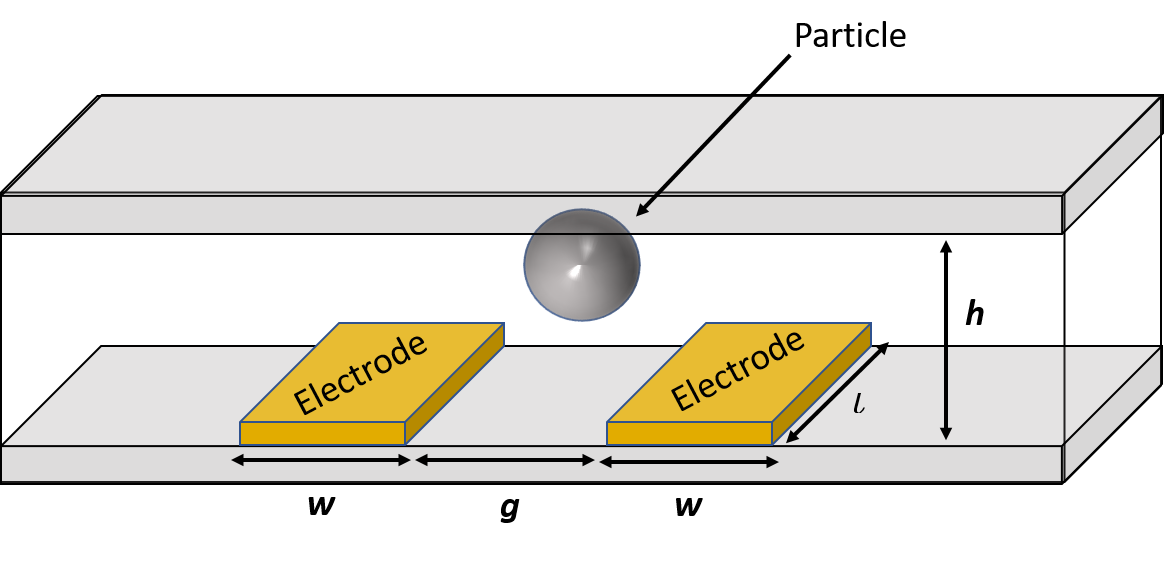
\includegraphics[width=0.7\textwidth]{images/cellAndElectrodes.png}
 \caption[Schematic diagram of simplified impedance sensor chamber.]{Schematic diagram of simplified impedance sensor chamber where w, $g$, and $l$ are the width, gap, and length of the electrodes respectively, and $h$ is the height of the chamber.}
 \label{fig:simplified_IS}
 \end{figure}
 
 

%%%%%%%%%%%%%%%%%%%%%%%%%%%%%%%%%%%%%
% Maxwell's Mixture Theory
%%%%%%%%%%%%%%%%%%%%%%%%%%%%%%%%%%%%%
\section{Maxwell's Mixture Theory}
 
 Maxwell's equation for the complex permittivity of a mixture is
  
  \begin{equation}
      \tilde{\epsilon}_{mix} = \tilde{\epsilon}_m\frac{1 + 2\Phi\tilde{f}_{CM}}{1-\Phi\tilde{f}_{CM}}
  \end{equation}
  
  \noindent where $\tilde{\epsilon}_{mix}$ is the complex permittivity of the mixture, $\tilde{\epsilon}_m$ is the complex permittivity of the medium, $\tilde{f}_{CM}$ is the Clausius Mossotti factor, and $\Phi$ is the volume fraction.
  
  \par The Clausius Mossotti factor is defined as 
  
  \begin{equation}
    \tilde{f}_{CM} = \frac{\tilde{\epsilon}_p - \tilde{\epsilon}_m}{\tilde{\epsilon}_p + 2\tilde{\epsilon}_m} 
  \end{equation}
  
  \noindent
  
  where $\tilde{\epsilon}_p$ is the complex permittivity of the particle and $\tilde{\epsilon}_m$ is the complex permittivity of the medium. 

 \begin{figure}[ht]
 \centering
 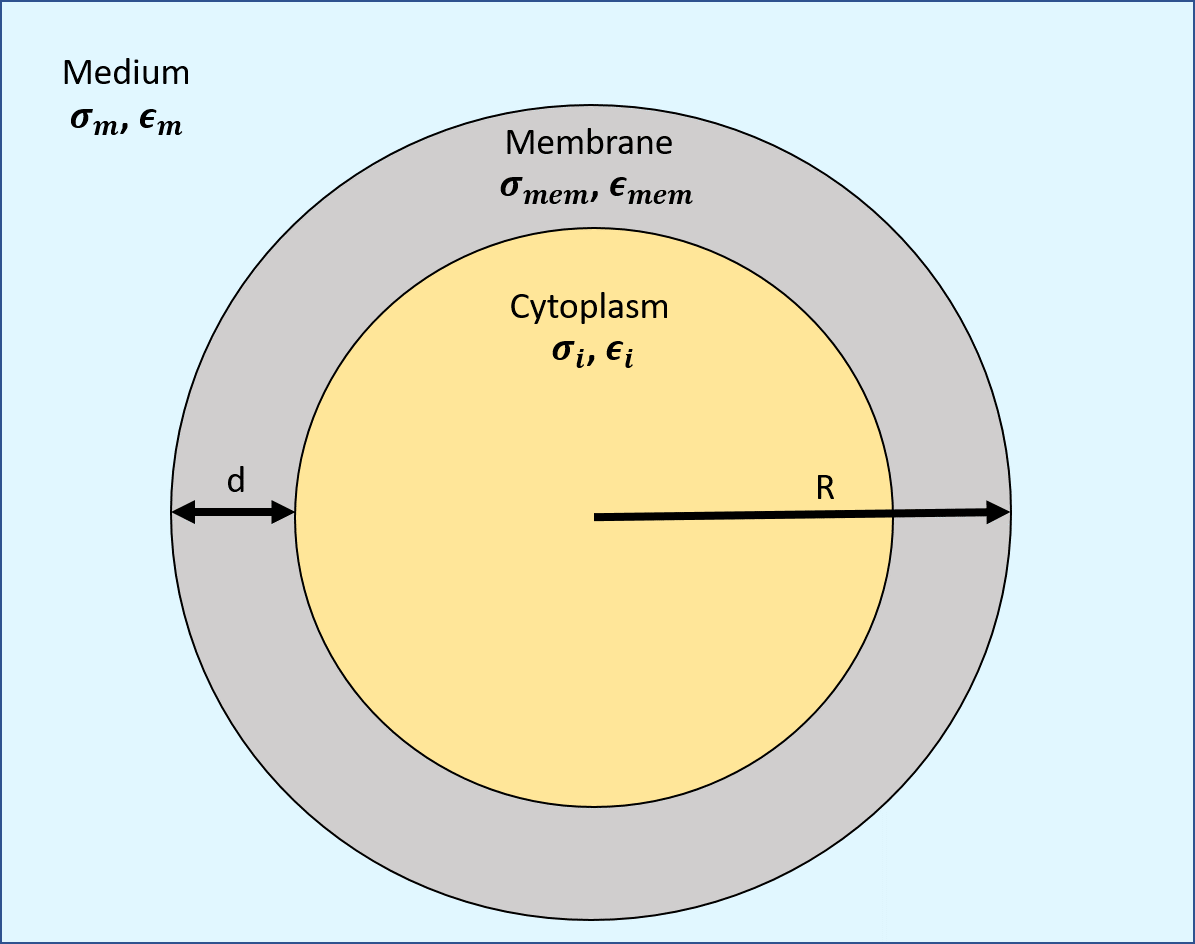
\includegraphics[width=0.7\textwidth]{images/singleShelledCell.png}
 \caption[Diagram of single shelled cell model.]{A diagram of a single shelled cell model where $\sigma_m$, $\epsilon_m$; $\sigma_{mem}$, $\epsilon_{mem}$; $\sigma_i$, and $\epsilon_i$ are the conductivity and permittivity of the medium, cell membrane, and cell cytoplasm respectively. $R$ and $d$ are the radius of the cell and membrane thickness respectively.}
 \label{fig:single_shell}
 \end{figure}

  \par The permittivity of the single shelled cell in figure \ref{fig:single_shell}, can be modelled as
  
  \begin{equation}
      \tilde{\epsilon}_p = \tilde{\epsilon}_{mem} 
      \frac{\gamma^3+2(\frac{\tilde{\epsilon}_i - \tilde{\epsilon}_{mem}}
      {\tilde{\epsilon}_i + 2\tilde{\epsilon}_{mem}})}{\gamma^3 - (\frac{\tilde{\epsilon}_i - \tilde{\epsilon}_{mem}}{\tilde{\epsilon}_i + 2\tilde{\epsilon}_{mem}})} \;\;\text{  with } 
      \gamma = \frac{R + d}{R} 
  \end{equation}
  
  \noindent where $\tilde{\epsilon}_i$ is the complex permittivity of the cytoplasm, $\tilde{\epsilon}_{mem}$ is the complex permittivity of the cell membrane, $R$ is the radius of the cell, and $d$ is the thickness of the cell membrane.

  
  The impedance of the mixture is
  
  \begin{equation}
    \tilde{Z}_{mix} = \frac{1}{jw\tilde{C}_{mix}}
    \label{eqn:impedance_with_cap}
  \end{equation}
  
  \noindent where $w$ is the angular frequency and $\tilde{C}_{mix}$ is the complex capacitance of the mixture and can be expressed as
  
  \begin{equation}
      \tilde{C}_{mix} = \tilde{\epsilon}_{mix} G_f
      \label{eqn:capacitance_mix}
  \end{equation}
  
  \noindent If equations \ref{eqn:impedance_with_cap} and \ref{eqn:capacitance_mix} are combined, we obtain
  
  \begin{equation}
    \tilde{Z}_{mix} = \frac{1}{jw\tilde{\epsilon}_{mix}G_f}
    \label{eqn:impedance_with_Gf}
  \end{equation}
  
  \par To find the value of the geometric factor $G_f$, the cell constant of the electrodes must be determined.
  
  
  %%%%%%%%%%%%%%%%%%%%%%%%%%%%%%%%%%%
  % Electrode Cell Constant
  %%%%%%%%%%%%%%%%%%%%%%%%%%%%%%%%%%%
  \section{Electrode Cell Constant}
  
  \par The cell constant $\kappa$ is defined as the proportionality factor between the measured resistance $R_b$ and the resistivity $\rho$ of a material.
  
  \begin{equation}
      R_b = \kappa \rho
      \label{eqn:cell_constant_proportionality}
  \end{equation}
  
  \noindent  Olthius related the measured resistance to capacitance in order to derive an analytic solution to cell constant \cite{olthuis_theoretical_1995}. 
  
  \par To find $R_b$ for two electrodes with an interspatial material, the measured resistance can be related to capacitance via Ohm's law and Maxwell's equation.
  
  \begin{equation}
      RC = \frac{\oiint \epsilon \boldsymbol{E} \cdot d\boldsymbol{S}}{\oiint \sigma\boldsymbol{E}\cdot d\boldsymbol{S}}
      \label{eqn:RC_integral}
  \end{equation}
  
  \noindent where $R$ and $C$ are the resistance and capacitance between the electrodes, $\epsilon$ is the product of the relative and vacuum permittivity, $\boldsymbol{E}$ is the electric field vector, and the integral is taken over a surface including one electrode.
  
  \par If the interspatial material is homogeneous and isotropic, then equation \ref{eqn:RC_integral} can be reduced to
  
  \begin{equation}
      RC = \frac{\epsilon}{\sigma}
      \label{eqn:RC}
  \end{equation}
  
  \par If we take $R_b = R$, we can combine equation \ref{eqn:RC} and \ref{eqn:cell_constant_proportionality} to express the cell constant in terms of capacitance.
  
  \begin{equation}
      \kappa = \frac{\epsilon}{C}
      \label{eqn:cell_constant_C}
  \end{equation}
  
   \begin{figure}[ht]
  \centering
  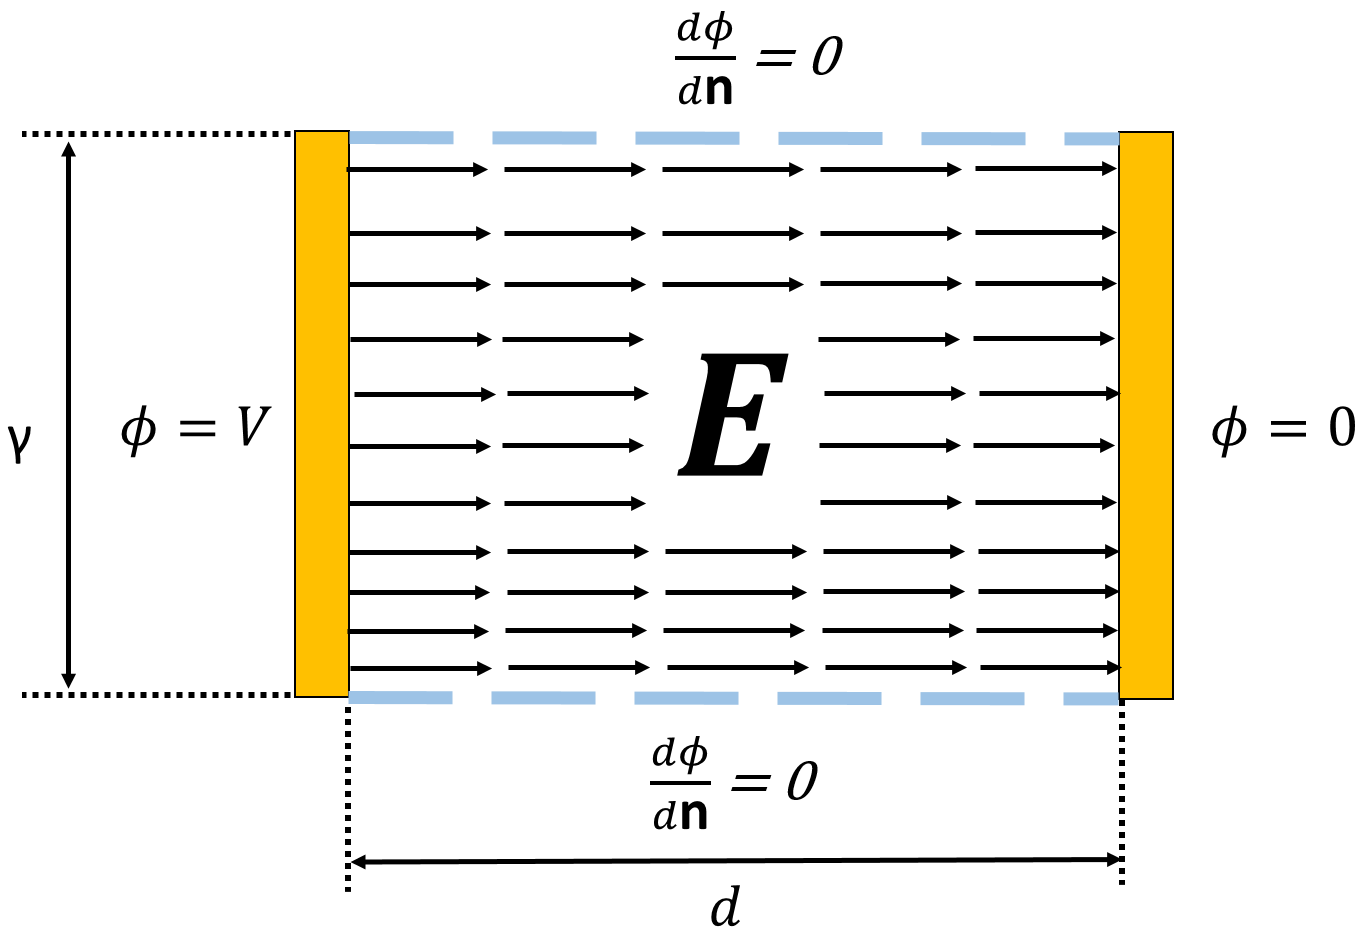
\includegraphics[width=0.7\textwidth]{images/capacitorNoFringe.png}
  \caption[Uniform electric field between parallel plates]{Uniform electric field between two parallel electrodes where $\boldsymbol{E}$ is the electric field, $\phi$ is the voltage, and $\frac{d\phi}{d\boldsymbol{n}}=0$ is the boundary condition of a perfect insulator. The dimensions of the capacitor are the electrode height $\gamma$, and the distance between the electrodes $d$.}
  \label{fig:parallel_capacitor}
  \end{figure}
  
  \par The capacitance of the two parallel plates with a uniform electrode field in figure \ref{fig:parallel_capacitor} is
  \begin{equation}
      C = \frac{\epsilon A}{d}
      \label{eqn:capacitor}
  \end{equation}
  
  \noindent where $A$ is the area of the plate and $d$ is the distance between the plates. Since $A = l\gamma$, where $l$ is the width, and $\gamma$ is the height of the electrode, the capacitance per unit width can be written as
  
  \begin{equation}
      C_l = \frac{\epsilon\gamma}{d} \;\;\;\text{where} \;\; C =l\, C_l
      \label{eqn:specific_capacitance}
  \end{equation}
  
  \par Returning to equation \ref{eqn:cell_constant_C}, and substituting equation \ref{eqn:specific_capacitance}, the cell constant can be expressed as 
  
  \begin{equation}
      \kappa = \frac{d}{\gamma \, l}
      \label{eqn:cell_constant}
  \end{equation}
  
  \noindent The geometric factor is related to the cell constant by 
  
  \begin{equation}
       G_f = (\kappa)^{-1}
       \label{geometric_cell}
  \end{equation}

  \noindent By combining equations \ref{eqn:cell_constant} and \ref{geometric_cell}, the geometric factor can be expressed as
  
  \begin{equation}
      G_f = \frac{\gamma l}{d}
      \label{eqn:geometric_constant}
  \end{equation}
  
  \par Equation \ref{eqn:geometric_constant} is the solution of the geometric constant for the electrode configuration in figure \ref{fig:parallel_capacitor}, but to find the geometric constant for any other configuration, including the coplanar electrode in figure \ref{fig:simplified_IS}, $d$ and $\gamma$ will need to be mapped to parameters in the other configuration. This will be accomplished in the next section with conformal transformations.
  
  
  %%%%%%%%%%%%%%%%%%%%%%%%%
  % Conformal Mapping
  %%%%%%%%%%%%%%%%%%%%%%%%%
  \section{Conformal Transformations}
  \label{app:conformal_mapping}
  
  \begin{figure}[h]
  \centering
  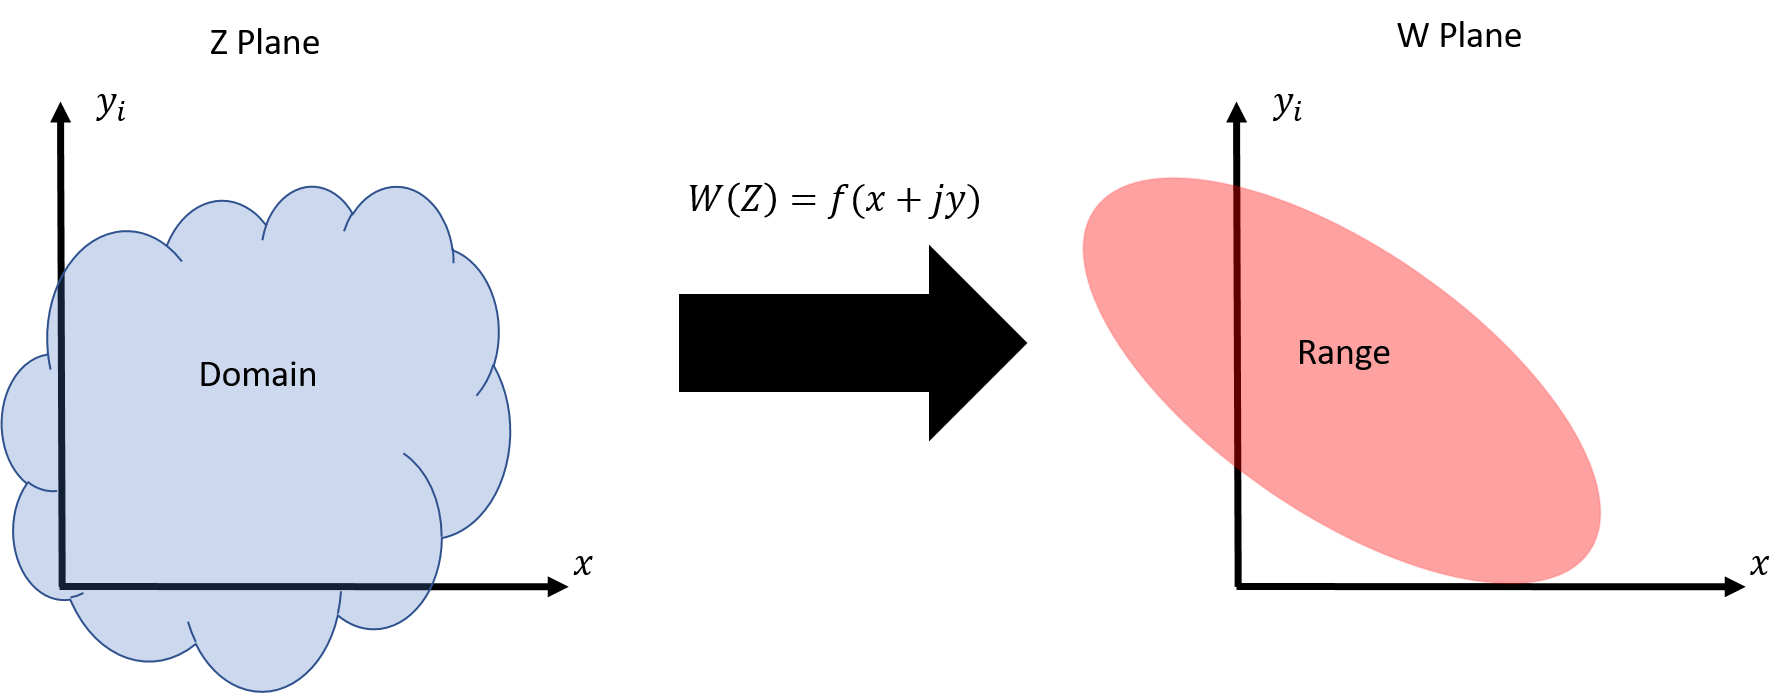
\includegraphics[width=\textwidth]{images/mapping.png}
  \caption[Illustration of complex mapping.]{An Illustration of complex mapping.}
  \label{fig:mapping}
  \end{figure}
  
  \par Let $z = x + j\,y$, where $j$ is the imaginary number $\sqrt{-1}$, then a function of $z$, such as $W(z) = u(x,y) + j\,v(x,y)$, can be considered a mapping of an area of one complex plane to an area in another complex plane (figure \ref{fig:mapping}). Conformal transformations are a special kind of mapping between two complex planes that preserves local angles. A mapping is conformal if it is composed of analytic functions, and as a consequent, fulfills the Cauchy-Rieman equations. Conformal mappings are extremely useful for solving problems in complicated domains by mapping the problem to a new domain where the problem is simplified. An example of a conformal mapping is $w(z) = tan(z)$, which maps an infinite vertical strip to a circle (figure \ref{fig:circleMapping}). 

   \begin{figure}[h]
    \centering
    \begin{subfigure}[b]{0.45\textwidth}
        \centering
        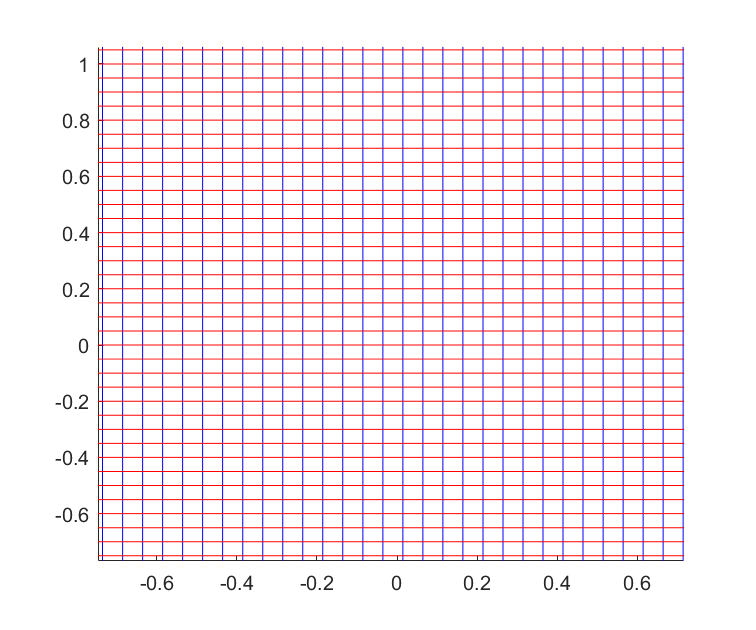
\includegraphics[width=\textwidth]{images/tanMappingStrip.png}
        \caption{Part of the partial infinite strip $-\pi/4<x<\pi/4$.}
    \end{subfigure}
    \hfill
    \begin{subfigure}[b]{0.45\textwidth}
        \centering
        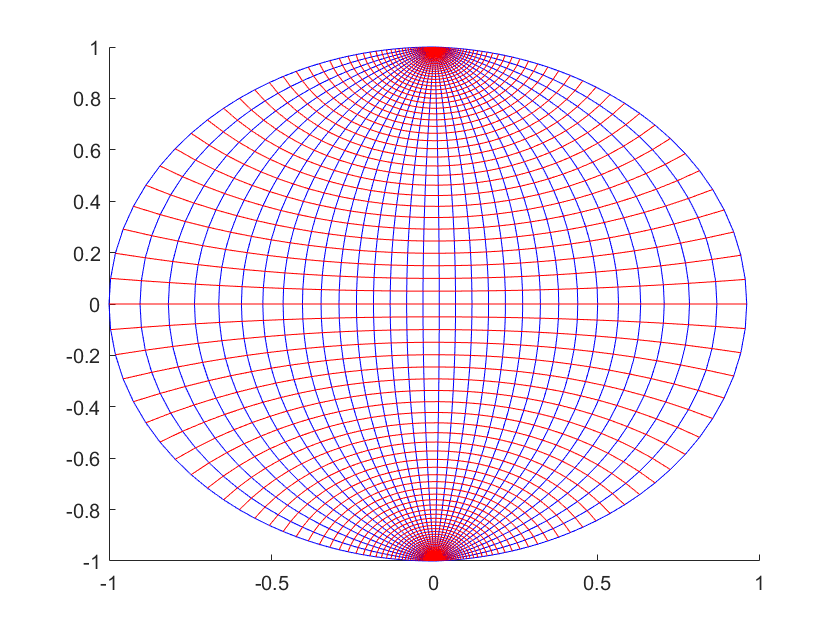
\includegraphics[width=\textwidth]{images/tanMapping.png}
        \caption{Mapping of the partial infinite vertical strip to a circle }
    \end{subfigure} 
    \caption[Conformal mapping of vertical strip to circle]{An example of conformal mapping by transforming a partial infinite vertical strip to a circle with the mapping $w(z) = tan(z)$.}
    \label{fig:circleMapping}
 \end{figure}
  
 
    \par Sun, Greene, et al. utilized the Schwartz-Christoffel transform to map the coplanar electrode configuration in figure \ref{fig:simplified_IS} to the configuration of parallel electrodes with uniform electrode fields in figure \ref{fig:parallel_capacitor} \cite{sun_analytical_2007}. The Schwartz-Christoffel formula is a powerful transform that allows the mapping of the upper complex T-plane ($y>0$) to the inside of a polygon. The formula is
    
    \begin{equation}
        Z = C_1 \int_{T_0}^T \prod^m_{r=1} (T - T_r)^{(\theta_r/\pi - 1)} dT + C_2
    \end{equation}
    
    \noindent where $Z$ is the interior of a polygon in the Z-plane with vertices $Z_1,\;Z_2,\;Z_3,\; ...,Z_m$ and angles $\theta_1,\;\theta_2,\;\theta_3,\; ...,\theta_m$ which correspond to the points $T_1,\;T_2,\;T_3,\; ...,T_m$ on the real axis of the T-plane. $C_1$ and $C_2$ are integration constants. The Schwartz-Christoffel transform has three degrees of freedom, and consequently, up to three points may be chosen arbitrarily. $T_0$ is the reference and is typically chosen at the origin.
    
    \par To find the geometric constant for coplanar electrodes, Schwartz-Christoffel transforms will be used to map the coplanar electrode geometry (Z-plane) to the upper complex plane (T-plane) and then to map the T-plane to the W-plane. The W-plane vastly simplifies the solution to the cell constant, and the goemetric constant can be solved for with equation \ref{eqn:geometric_constant}. 
    
    \begin{figure}[h]
        \centering
        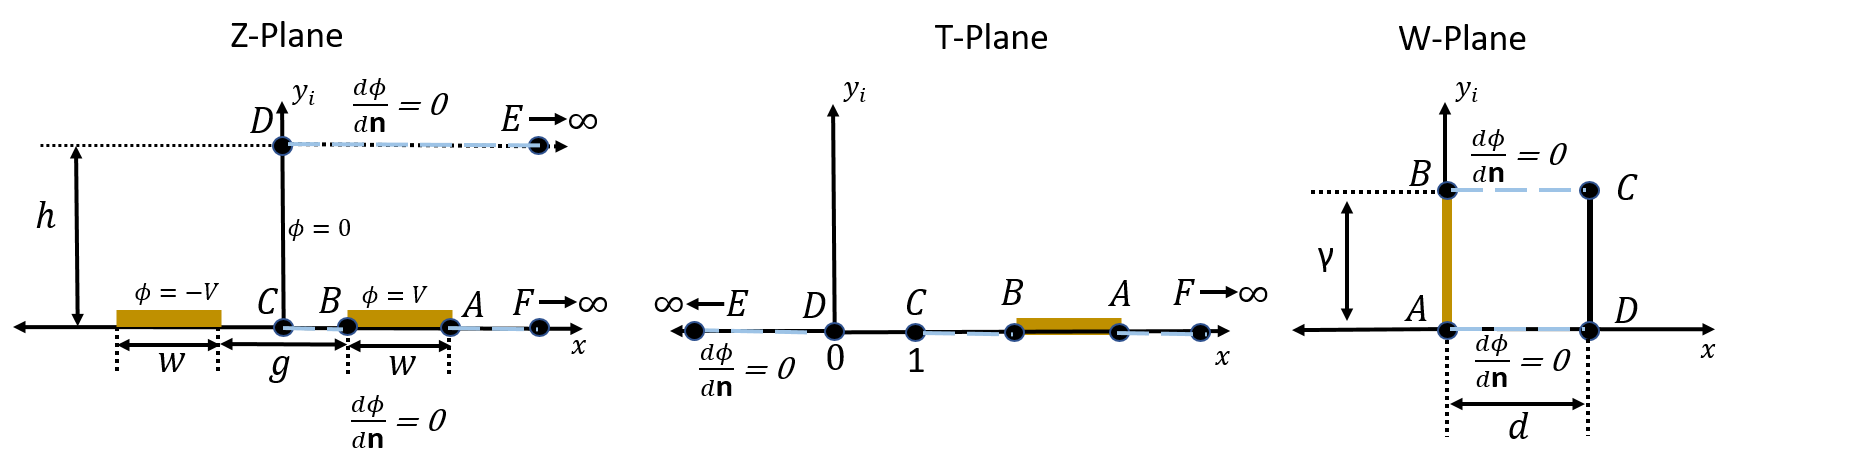
\includegraphics[width=\textwidth]{images/scmPlanes.png}
        \caption[Diagrams of coplanar electrodes through Schwartz-Christoffel mapping]{Diagrams of coplanar electrodes through Schwartz-Christoffel mapping where the Z-plane contains the physical dimensions of the electrode configuration, the T-Plane links the Schwartz-Christoffel mappins of Z and W plane, and the W-plane represents the parallel electrodes producing a uniform electrode field.}
        \label{fig:scm_planes}
    \end{figure}
    
    
\subsection{Schwartz-Christoffel Transform: T to Z Mapping}

  \par Mapping the T-plane to the Z-plane, point $C$ and $D$ will be chosen as the polygon corners with angles of $\pi/2$.  
  \begin{equation}
      Z = C_1\int (T-T_c)^{-1/2}(T-T_D)^{-1/2}dT + C_2
      \label{eqn:SCM_ZT_int}
  \end{equation}
 \noindent To integrate
 \begin{flalign*}
    &\int (T-T_D)^{-1/2}(T-T_C)^{-1/2}dT&\\
 \end{flalign*}
 \noindent Substitute $u = (T-T_C)^{1/2}\;$ with $\;du = \frac{1}{2} (T-T_C)^{-1/2} \, dT$
\begin{flalign*}
    &= 2\int \frac{du}{\sqrt{T-T_D}}\;\;\;\;\; \text{with}\;\;  T = u^2 + T_C&  \\
    \\
    &= 2\int \frac{du}{\sqrt{u^2 + T_C - T_D}}& \\
    \\
    &= 2\int \frac{\sqrt{T_C-T_D}}{\sqrt{\frac{u^2}{T_C-T_D}+1}}\;\;du&
\end{flalign*}

\noindent substitute $t = \frac{u}{\sqrt{T_C - T_D}};\;\;dt = \frac{du}{\sqrt{T_C-T_D}}$
\begin{flalign*}
    &=2\int \frac{dt}{\sqrt{t^2+1}}&
\end{flalign*}


\noindent Substitute $t = tan(s)$\;\; with $dt=\sec^2s$
\begin{flalign*}
    \allowdisplaybreaks
    &= 2\int \sec(s) ds& \\
    \\
    &= 2\ln(\tan(s) + \sec(s))&\\
    \\
    &= 2\ln(t + \sec(\arctan(t)))&
    \end{flalign*}
    \begin{flalign*}
    &= 2\ln(t + \sqrt{s^2+1})&\\
    \\
    &= 2\ln \Bigg( \frac{u}{\sqrt{T_C-T_D}}+\sqrt{\frac{u^2}{T_C-T_D}+1}\Bigg)&\\
    \\
    &= 2\ln \Bigg( \frac{u}{\sqrt{T_C-T_C}} + \sqrt{\frac{u^2+T_C-T_D}{T_C-T_D}}\Bigg)&\\
    \\
    &= 2\ln \Bigg( \sqrt{\frac{T-T_C}{T_C-T_D}} + \sqrt{\frac{T-T_D}{T_C-T_D}}\Bigg)&
\end{flalign*}

\noindent Add the integration constants from equation \ref{eqn:SCM_ZT_int} and combine $(T_C + T_D)^{-1/2}$ in $C_2$, then
\begin{equation}
Z = 2C_1\ln \Bigg( \sqrt{T-T_C} + \sqrt{T-T_D} \Bigg) + C_2
\end{equation}

\noindent The points $T_C$ and $T_D$ will be chosen to be 1 and 0 respectively
\begin{equation}
    Z = 2C_1\ln \Bigg( \sqrt{T-1} + \sqrt{T} \Bigg) + C_2
    \label{eqn:ZT_with_constants}
\end{equation}
  
 \noindent The integration constants can be solved by relationships in the coordinates between the Z-plane and T-plane. 
 
 \noindent For point C, $Z_C = 0$ and $T_C=1$,
 \begin{flalign*}
 &0=2C_1(0) + C_2&\\
 &C_2=0&
 \end{flalign*}
 \noindent For point D, $Z_D = jh$ and $T_D=1$,
 \begin{flalign*}
 jh &= 2C_1\ln(j)&\\
 jh &= 2C_1(\frac{\pi}{2} j)&\\
 C_1 &= \frac{h}{\pi}&
 \end{flalign*}
 
 \noindent After substituting the values of the integration constants into equation \ref{eqn:ZT_with_constants},
 
 \begin{equation}
     Z = \frac{2h}{\pi}\ln\Big(\sqrt{T-1} + \sqrt{T}\Big)
     \label{eqn:TZ}
 \end{equation}
 
    \begin{figure}[h]
    \centering
    \begin{subfigure}[t]{0.45\textwidth}
        \centering
        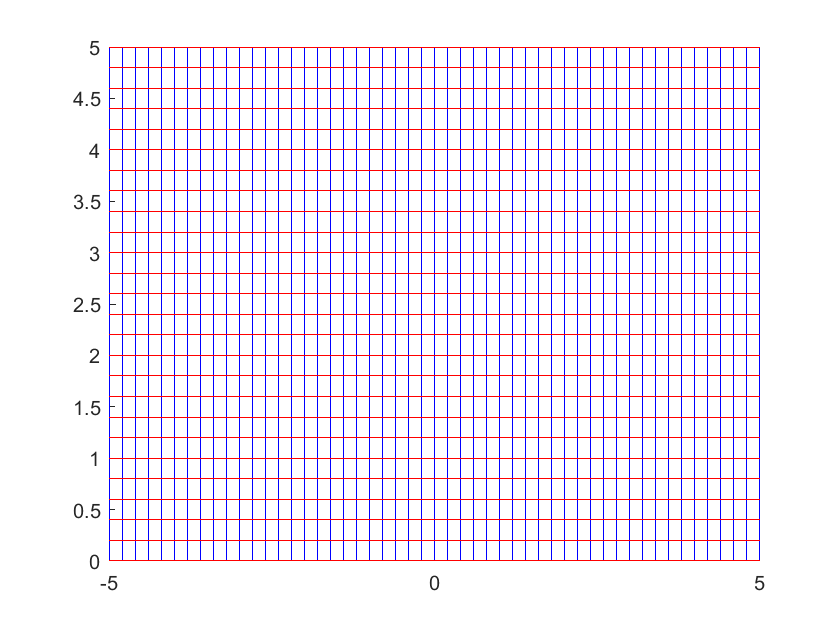
\includegraphics[width=\textwidth]{images/TtoZ_strip.png}
        \caption{Part of upper complex T-Plane}
    \end{subfigure}
    \hfill
    \begin{subfigure}[t]{0.45\textwidth}
        \centering
        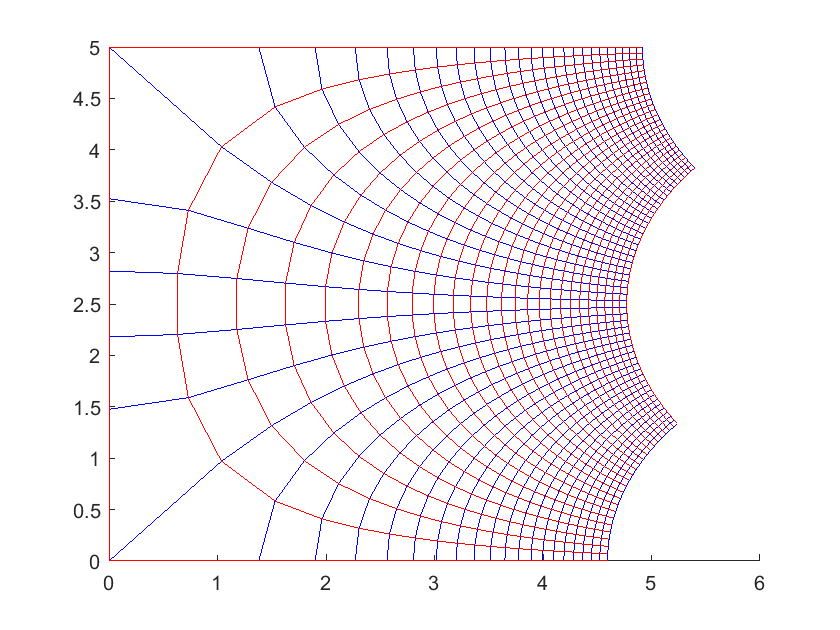
\includegraphics[width=\textwidth]{images/TtoZ_map.png}
        \caption{Mapping of the part of the T-plane to the polygon in the Z-plane}
    \end{subfigure} 
    \caption[Mapping of the T-plane to the inside of the open polygon in the Z-Plane]{Mapping of the T-plane to the inside of the open polygon in the Z-Plane outlined by the points $F$, $C$, $D$, and $E$ in the Z-plane. Equation \ref{eqn:TZ} is the mapping function.} 
    \label{fig:T_to_Z_mapping}
 \end{figure}
 
 \noindent The mapping from the Z-plane to the T-plane can be found by solving for T in equation \ref{eqn:TZ}.
 \begin{flalign*}
 Z &= \frac{2h}{\pi}\ln\Big(\sqrt{T-1} + \sqrt{T}\Big)&\\
 \\
 \frac{Z\pi}{2h} &= \ln\Big(\sqrt{T-1} + \sqrt{T}\Big)&
 \end{flalign*}
 
 \noindent And utilizing the inverse hyperbolic identity
 \begin{flalign*}
 \arccosh(z) &= \ln\Big(z + \sqrt{z-1}\sqrt{z+1}\Big)&\\
 \\
 \arccosh(z) &= \ln\Big(z + \sqrt{z^2-1}\Big)&
 \end{flalign*}
 \noindent Substitute $z = \sqrt{T}$
 \begin{flalign*}
 \arccosh(\sqrt{T}) &= \ln\Big(\sqrt{T} + \sqrt{T-1}\Big)&
 \end{flalign*}
 \noindent Then $T$ can be solved for as
 \begin{equation}
     T = \cosh^2\bigg(\frac{z\pi}{2h}\bigg)
     \label{eqn:ZT}
 \end{equation}
 
     \begin{figure}[h]
    \centering
    \begin{subfigure}[t]{0.45\textwidth}
        \centering
        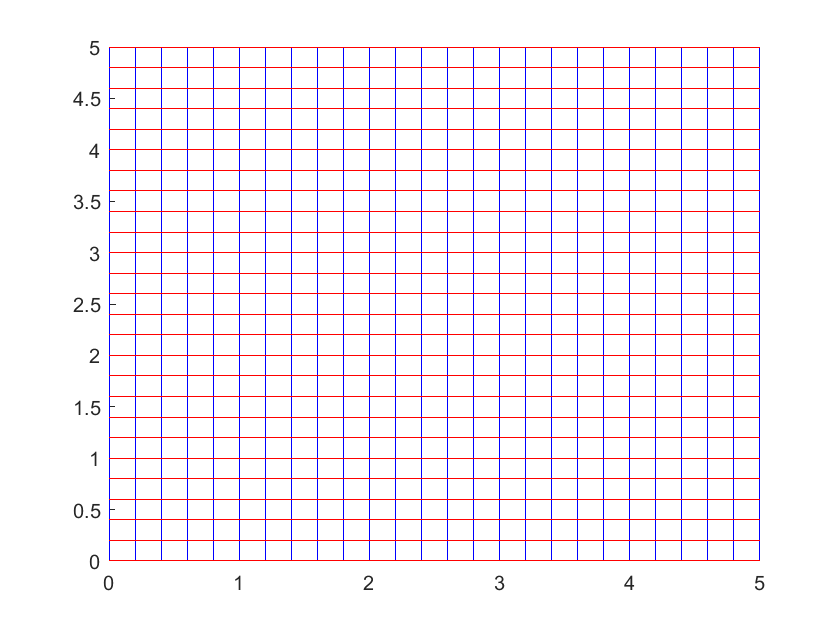
\includegraphics[width=\textwidth]{images/ZtoT_strip.png}
        \caption{Part of the open polygon in the Z-plane.}
    \end{subfigure}
    \hfill
    \begin{subfigure}[t]{0.45\textwidth}
        \centering
        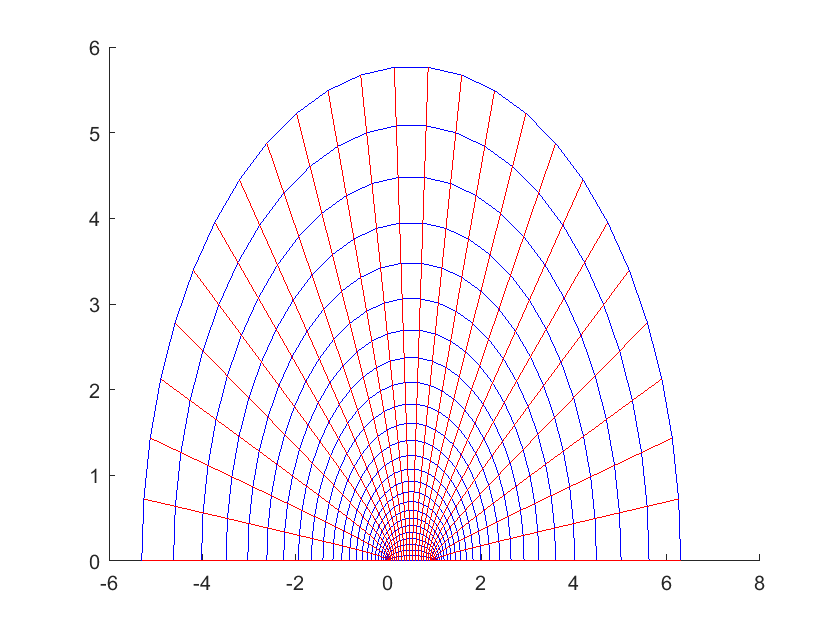
\includegraphics[width=\textwidth]{images/ZtoT_map.png}
        \caption{Mapping of part of the polygon in the Z-plane to the T-plane.}
    \end{subfigure} 
    \caption[Mapping of the open polygon in the Z-Plane to the T-plane.]{Mapping of the open polygon in the Z-Plane outlined by the points $F$, $C$, $D$, and $E$ to the T-plane. Equation \ref{eqn:ZT} is the mapping function.} 
    \label{fig:Z_to_T_mapping}
 \end{figure}

\subsection{Schwartz-Christoffel Transform: W to T Mapping}
 
 \par Mapping the T-plane to the W-Plane, points $A$, $B$, $C$, and $D$, will be chosen as the polygon corners with angles of $\pi/2$.
 \begin{equation}
    W = D_1 \int (T-T_A)^{-1/2}(T-T_B)^{-1/2}(T-T_C)^{-1/2}(T-T_D)^{-1/2}\;dT + D_2
    \label{eqn:scm_wt_int}
 \end{equation}
 
 \noindent Since equation \ref{eqn:scm_wt_int} is an integral of a rational function with a root of a quartic polynomial, the function can be rewritten as an elliptic integral \cite{i.s._gradshteyn_table_1980}.
 
 \begin{equation}
     W = D_3F(v,k) + D_2
 \end{equation}
 \begin{equation}
    D_3 = \frac{2D_1}{\sqrt{(T_A - T_C)(T_B-T_D)}}
 \end{equation}
 
 \begin{equation}
     v = \arcsin\sqrt{\frac{(T_B-T_D)(T-T_A)}{(T_A-T_D)(T-T_B)}}
 \end{equation}
 
 \begin{equation}
     k = \sqrt{\frac{(T_B-T_C)(T_A-T_D)}{(T_A-T_C)(T_B-T_D)}}
 \end{equation}
 \noindent Where $F(v,k)$ is the incomplete elliptic integral of the first kind, and can be expressed as
 \begin{equation}
     F(v,k) = \int^v_0 \frac{d\alpha}{\sqrt{1 - k^2\sin^2\alpha}}
 \end{equation}
 \noindent Where $v$ and $k$ are referred to as the amplitude and modulus respectively.
 
 \noindent Solving for the integral constants, for point A, $W_A = 0$ and $v = 0$
 \begin{flalign*}
    0 &= D_3F(0,k) + D_2&\\
    F(0,k) &= 0&\\
    D_2 &= 0&
 \end{flalign*}

\noindent For point $D$, $W_D = d$ and $v = \pi/2$
 \begin{flalign*}
 d &= D_3F(\pi/2, k)&\\
 D_3 &= \frac{d}{F(\pi/2,k)}&\\
 D_3 &= \frac{d}{K(k)}&
 \end{flalign*}

\noindent Where $K(k)$ is the complete elliptic integral and is expressed as 
 \begin{equation}
     K(k) = \int_0^{\pi/2} \frac{d\alpha}{1 - k^2\sin^2(\alpha)}
 \end{equation}
 
 \noindent For point $B$, $W_B = j\gamma$ and $\lim_{T\to ^-T_B} v = \arcsin{(i\infty)}$
 \begin{flalign*}
 j\gamma &= D_3F(j\infty, k)&\\
 D_3 &= \frac{F(j\infty,k)}{j\gamma}&
 \end{flalign*}
 
 \noindent Equating the two solutions for $D_3$, the Geometric factor (equation \ref{eqn:geometric_constant}) in the W-Plane can be mapped to T-plane and, using equation \ref{eqn:ZT}, mapped to the Z-plane.
 
 \begin{equation}
     D_3 = \frac{d}{K(k)} = \frac{j\gamma}{\lim_{v\to j\infty}F(v,k)} 
     \label{eqn:prep_D3}
 \end{equation}
 \begin{equation}
     G_f = \frac{\gamma l}{2\,d} = \frac{\lim_{v\to i\infty}F(v,k)l}{j\,2\,K(k)}
     \label{eqn:geometric_constant_mapping}
 \end{equation}
 
 \noindent A constant of two appears in the denominator of \ref{eqn:geometric_constant_mapping} since the conformal mapping takes advantage of symmetry and only accounts for half of the disance between the electrodes in the W-plane (figure \ref{fig:scm_planes}).
 

 \par However, the expression $\lim_{v \to i\infty}F(v,k)$ is difficult to handle, but by using the imaginary-argument transform, it can be shown that $\lim_{v\to j\infty} F(v,k) = iK(k')$. 
 
  \subsection*{Proof That $\displaystyle\boldsymbol{\lim_{v\to j\infty} F(v,k) = iK(k')}$}
 
 The Imaginary-argument transform states that
 \begin{equation}
     F(i\phi,k) = iF(\psi, k')\;\; \text{with} \;\; \sinh\phi = \tan\psi
     \label{eqn:imaginary_argument}
 \end{equation}
 
 \noindent Where $k' = \sqrt{1 - k^2}$ and is called the complement modulus. Starting with the definition of $\arcsin x$:
 \begin{flalign*}
    \arcsin{x} =& -j\Log(jx + (1-x^2)^{1/2})&
 \end{flalign*}
 
 \noindent and with $w$ defined as $w = jx$, where $x$ is a real number, then
 \begin{flalign*}
  jw + (1 - w^2)^{1/2} &= (1+x^2)^{1/2} - x&
 \end{flalign*}
 
 \noindent and taking the limit as $x\to\infty$
 \begin{flalign*}
  \lim_{x\to\infty}& \;\; (1+x^2)^{1/2} - x&\\
  =\lim_{x\to\infty}& \;\; \frac{(\frac{1}{x^2}+1)^{1/2}}{x^{-1}}& \text{Apply L'Hopitals}\\
  =\lim_{x\to\infty}& \;\; \frac{1}{x(\frac{1}{x^2}+1)^{1/2}}&\\
  =& \;\; 0&
 \end{flalign*}

 \noindent Which implies that 
  \begin{flalign*}
  \lim_{w\to j\infty} \Log(jw + (1-w^2)^{1/2}) &= -\infty&
 \end{flalign*}
 
 \noindent For convenience, the following will be defined:
 
 \begin{equation}
     Q(w) = \Log(jw + (1-w^2)^{1/2})
 \end{equation}
 \begin{equation}
     \lim_{w\to j\infty} Q = -\infty
 \end{equation}
 
 \noindent And now it can be stated that $\arcsin(w) = -jQ$. Returning to the imaginary-argument transform (equation \ref{eqn:imaginary_argument}), 
 \begin{flalign*}
  F&(-jQ,k) = F(\psi, k')&\\
  \psi & = \arctan\Big(\sinh(-Q)\Big)&\\
  \psi & = \arctan\Big(\frac{1}{2}(e^{-Q}-e^{Q})\Big)&\\
  \\
  \psi & = \frac{j}{2}\Log\Big(\frac{j+\frac{1}{2}(e^{-Q}-e^{Q})}{j-\frac{1}{2}(e^{-Q}-e^{Q})}\Big)&\\
  \\
  \psi & = \frac{j}{2} \bigg[\ln\bigg|\frac{j+\frac{1}{2}(e^{-Q}-e^{Q})}{j-\frac{1}{2}(e^{-Q}-e^{Q})} \bigg| + j\,arg\Big(\frac{j+\frac{1}{2}(e^{-Q}-e^{Q})}{j-\frac{1}{2}(e^{-Q}-e^{Q})}\Big)\bigg]
 \end{flalign*}
 \noindent Where $\text{arg}(x+jy)$ is the angle of the vector $<x,y>$ with respect to the positive $x$ axis. 
 \noindent It can be noted that 
 \begin{flalign*}
 \Big|\frac{jy-x}{jy-x}\Big| &= \frac{|jy-x|}{|jy-x|}&\\
 \frac{|jy-x|}{|jy-x|} &= \frac{\sqrt{x^2+y^2}}{\sqrt{x^2+y^2}}&\\
 \ln\frac{\sqrt{x^2+y^2}}{\sqrt{x^2+y^2}} &= 0
 \end{flalign*}
 
 \noindent Returning to the solution of $\psi$,
 \begin{flalign*}
   \psi & = \frac{j}{2} \bigg[\ln\bigg|\frac{j+\frac{1}{2}(e^{-Q}-e^{Q})}{j-\frac{1}{2}(e^{-Q}-e^{Q})} \bigg| + j\,arg\Big(\frac{j+\frac{1}{2}(e^{-Q}-e^{Q})}{j-\frac{1}{2}(e^{-Q}-e^{Q})}\Big)\bigg]&\\
   \\
    \psi & = \frac{j}{2} \bigg[ j\,\text{arg}\Big(\frac{j+\frac{1}{2}(e^{-Q}-e^{Q})}{j-\frac{1}{2}(e^{-Q}-e^{Q})}\Big)\bigg]&
 \end{flalign*}
 
 \noindent And then letting $Q \to -\infty$
 \begin{flalign*}
    \psi & = \frac{j}{2} \bigg[ j\,\text{arg}\Big( \lim_{Q\to -\infty}  \frac{j+\frac{1}{2}(e^{-Q}-e^{Q})}{j-\frac{1}{2}(e^{-Q}-e^{Q})}\Big)\bigg]& \text{Apply L'Hopital's rule}\\
    \\
    \psi & = \frac{j}{2} \bigg[ j\,\text{arg}\Big( \lim_{Q\to -\infty}  \frac{\frac{d}{dQ}\frac{1}{2}(e^{-Q}-e^{Q})}{-\frac{d}{dQ}\frac{1}{2}(e^{-Q}-e^{Q})}\Big)\bigg]&\\
    \\
    \psi & = \frac{j}{2} \bigg[ j\,\text{arg}(-1)\bigg]&\\
    \\
    \psi & = \frac{\pi}{2}&
 \end{flalign*}
 
 \noindent showing that, with equation \ref{eqn:imaginary_argument},
 
 \begin{equation}
     \lim_{v\to j\infty} F(v,k) = jK(k')
 \end{equation}
 
 \noindent Returning to the mapping of the geometric factor (equation \ref{eqn:prep_D3}, and \ref{eqn:geometric_constant_mapping}), $D_3$ and $G_f$ can be expressed as
 \begin{equation}
     D_3 = \frac{d}{K(k)} = \frac{\gamma}{K(k')}
     \label{eqn:D3}
 \end{equation}
 \begin{equation}
     G_f = \frac{2\,K(k)}{K(k')}
     \label{eqn:Gf}
 \end{equation}
 
 \section{Solution to the Electric Field}
 \label{app:analytic_electric_field}
 
 \par Now with Z-T and T-W mappings, the solution of the electric field in the W-plane can be mapped to the Z-plane. The mapping of the electric field can be expressed as 
 
 \begin{equation}
     \boldsymbol{E_z} = -\nabla \phi_z \;\;\text{with} \;\;\;\nabla \phi_z = \nabla \phi_w \overline{\frac{dW}{dZ}}
     \label{eqn:ZtoW_efield}
 \end{equation}
 
 \noindent Where $\nabla \phi$ is the gradient of potential and $\overline{\frac{dW}{dZ}}$ is the conjugate of the derivative of $W$ with respect to $Z$ \cite{schinzinger_conformal_2012}.
 
 \par Applying the chain rule to equation \ref{eqn:ZtoW_efield}, the electric field mapping is expressed as
 
 \begin{equation}
    \boldsymbol{E_z} =- \nabla \phi_w \overline{\frac{dW}{dT}\frac{dT}{dZ}}
    \label{eqn:ZtoW_efield_chain}
 \end{equation}
 
 The gradient of $ \phi_w$ can be reduced to $\frac{d}{dx} \phi_w$ since the electric potential in the W-plane is independent of the $y$ and $z$ direction (figure \ref{fig:scm_planes}). The electric potential and electric field in the W-plane can be expressed as 
 
 \begin{equation}
    \phi_w = V\Big(1-\frac{x}{d}\Big)
 \end{equation}
 \begin{equation}
     E_w = -\nabla \phi_w = \frac{V}{d}
     \label{eqn:phi_w}
 \end{equation}
 
 \noindent $\frac{dW}{dT}$ can be found by integrating equation \ref{eqn:scm_wt_int}.
 
 \begin{equation}
     \frac{dW}{dT} = \frac{d}{K(k)}\frac{(T_A - T_C)^{1/2}(T_B-T_D)^{1/2}}{(T-T_A)^{1/2}(T-T_B)^{1/2}(T-T_C)^{1/2}(T-T_D)^{1/2}}
     \label{eqn:dwdt}
 \end{equation}
 
 
 \noindent And $\frac{dT}{dz}$ can be found by integrating equation \ref{eqn:ZT}.
 \begin{flalign*}
 T &= \cosh^2\Big(\frac{Z\pi}{2h}\Big)&\\
 \\
 \frac{dT}{dZ} &= 2\cosh\Big(\frac{Z\pi}{2h}\Big)\sinh\Big(\frac{Z\pi}{2h}\Big)\frac{\pi}{2h}& \text{Substitute equation \ref{eqn:TZ}}\\
 \\
  \frac{dT}{dZ} &= \frac{\pi}{h}\cosh\Big(\ln(\sqrt{T-1}+\sqrt{T})\Big)\sinh\Big(\ln(\sqrt{T-1}+\sqrt{T})\Big)&
 \end{flalign*}
 
 \noindent And then applying the inverse cosh and sinh log relations, 
 \begin{flalign*}
 \arccosh x &= \ln(x + \sqrt{x^2-1})&\\
 \arcsinh x &= \ln(x + \sqrt{x^2+1})&
 \end{flalign*}
 
 \begin{equation}
     \frac{dT}{dZ} = \frac{\pi}{h}(\sqrt{T-T_D})(\sqrt{T-T_C})
     \label{eqn:dtdz}
 \end{equation}
 
 \par Combining equations, \ref{eqn:ZtoW_efield_chain}, \ref{eqn:phi_w}, \ref{eqn:dwdt}, and \ref{eqn:dtdz}, the electric field for the coplanar electrodes can be expressed as equation \ref{eqn:Ez} and is depicted in figure \ref{fig:Ez}
 
 \begin{equation}
    E_z = \overline{\frac{\pi V}{2hK(k)} \frac{\sqrt{(T_A-T_C)(T_B-T_D)}}{\sqrt{(T-T_A)(T-T_B)}}}
    \label{eqn:Ez}
 \end{equation}
 
 
     \begin{figure}[h]
        \centering
        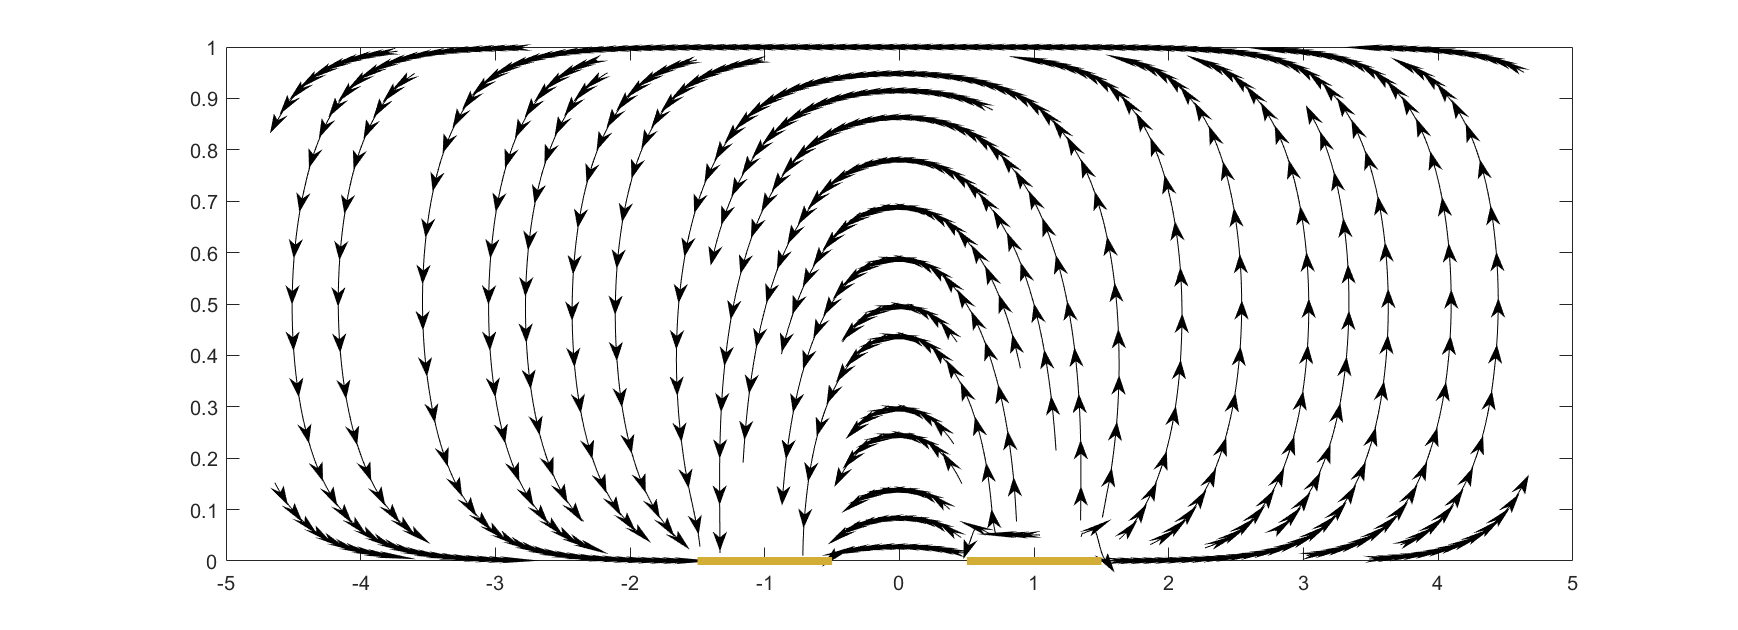
\includegraphics[width=\textwidth]{images/Ez.png}
        \caption[Electric Field for Coplanar Electrodes]{The electric field for coplanar electrodes as defined by equation \ref{eqn:Ez}.}
        \label{fig:Ez}
    \end{figure}